% Compilazione: pdflatex -jobname=statistica_tex statistica.tex
\documentclass[11pt,a4paper]{article}
\usepackage[utf8]{inputenc}\usepackage[T1]{fontenc}\IfFileExists{italian.ldf}{\usepackage[italian]{babel}}{\usepackage[english]{babel}}\usepackage{amsmath,amssymb,geometry,tikz}\geometry{margin=2cm}\setlength{\parindent}{0pt}\setlength{\parskip}{5pt}
\newcommand{\pagina}[1]{\clearpage}
\emergencystretch=3em
\begin{document}
% Pagina originale 1
\section*{Legenda}
\textbf{1. Statistica descrittiva}: popolazione, campione, bias, variabile, frequenza, diagramma a barre, diagramma a torta, dati raggruppati in classi, valori di sintesi: moda, media, varianza, quartili, percentili, quantili, retta di regressione lineare, covarianza, coefficiente di correlazione lineare, coefficiente di determinazione.

\textbf{2. Probabilità}: spazio degli eventi elementari, evento, collezione di tutti gli eventi, proprietà delle collezioni, misura di probabilità, principio di inclusione/esclusione, calcolo combinatorio (disposizione con ripetizioni, disposizione senza ripetizioni, permutazione, combinazione semplice), paradosso del compleanno, probabilità condizionata, teorema della probabilità totale, teorema di Bayes, problema di Monty Hall, eventi indipendenti, variabili aleatorie, legge di una variabile aleatoria, valore atteso, LOTUS, varianza, covarianza, vettori aleatori, funzioni di vettori aleatori, leggi note. Leggi discrete: Bernoulli $Be(p)$, binomiale $B(n,p)$, Poisson $\mathcal P(\lambda)$, geometrica $Geo(p)$. Leggi continue: uniforme $U(a,b)$, esponenziale $Exp(\lambda)$, gamma $Gamma(\alpha,\lambda)$, normale $\mathcal N(\mu,\sigma^2)$. Vettori aleatori continui, variabili aleatorie indipendenti.

\textbf{3. Statistica inferenziale}: definizioni, obiettivi, legge dei grandi numeri, teorema del limite centrale, intervalli di confidenza (I.C.), leggi continue per analisi inferenziale (chi-quadro $\chi^2(n)$, tStudent $t(n)$), I.C. unilaterali, test di ipotesi, p-value.
% Pagina originale 2
\pagina{2}\section*{Statistica descrittiva}
\textbf{Popolazione}: l'insieme contenente tutte le unità statistiche che saranno esaminate (in parte) per l'analisi statistica.

\textbf{Campione}: sottoinsieme della popolazione contenente tutte le unità statistiche esaminate.

\textbf{Bias}: è un errore che si commette effettuando un campionamento non rappresentativo della popolazione. Esempio: survivorship bias.

\textbf{Variabile}: l'oggetto di studio dell'analisi statistica. Può essere qualitativa (descrittiva; appartenenza ad una classe), quantitativa (discreta; continua).

\textbf{Frequenza}. Siano $x_1,x_2,\ldots,x_n$ dati del campione con $v_1,v_2,\ldots,v_k$ valori assunti dalle variabili (range). $f_j$ è il numero di volte in cui $x_i=v_j$:
\[f_j=\#\{i=1,\ldots,n:x_i=v_j\},\qquad\sum_{j=1}^k f_j=n.\]
\[p_j=\frac{f_j}{n},\qquad\sum_{j=1}^k p_j=1.\]
$f_j$: frequenza assoluta; $p_j$: frequenza relativa. Quindi le frequenze di variabili qualitative e quantitative discrete possono produrre dei grafici a barre e a torte.
% Pagina originale 3
\pagina{3}\textbf{Diagramma a barre delle frequenze assolute e relative}.
\begin{center}\begin{tikzpicture}[scale=.7]\draw[->](0,0)--(5,0) node[right]{$v_j$};\draw[->](0,0)--(0,4) node[above]{$f_j$};\foreach \x/\h/\v in {1/1.5/1,2/3/2,3/2.3/3}{\draw(\x,0) rectangle +(0.5,\h);\node[below] at (\x,0){$v_\v$};}\node at (7,2){$\longleftrightarrow$ scala $1/n$};\begin{scope}[xshift=10cm]\draw[->](0,0)--(5,0) node[right]{$v_j$};\draw[->](0,0)--(0,4) node[above]{$p_j$};\foreach \x/\h/\v in {1/1.5/1,2/3/2,3/2.3/3}{\draw(\x,0) rectangle +(0.5,\h);\node[below] at (\x,0){$v_\v$};}\end{scope}\end{tikzpicture}\end{center}
\textbf{Diagramma a torta}: non conta l'ordine. Gli angoli dei settori sono $\theta_j=p_j\,2\pi$, $\sum_{j=1}^n\theta_j=2\pi$.
\begin{center}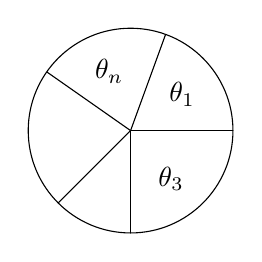
\begin{tikzpicture}\draw(0,0) circle(1.3);\foreach \a in {0,70,145,225,270}{\draw(0,0)--(\a:1.3);}\node at (35:.8){$\theta_1$};\node at (110:.8){$\theta_n$};\node at (310:.8){$\theta_3$};\end{tikzpicture}\end{center}
\textbf{Dati raggruppati in classi}. Un esempio di classe di dati è un intervallo:
\[I_j=[a_j,b_j),\quad I_{j+1}=[a_{j+1},b_{j+1}),\qquad b_j=a_{j+1}.\]
\[\bigcup_j I_j=I\quad\land\quad\bigcap_j I_j=\varnothing,\qquad f_j=\#\{i=1,\ldots,n:x_i\in I_j\}.\]
Per questo tipo di variabile uso l'istogramma (delle frequenze relative).
% Pagina originale 4
\pagina{4}Non è regolamentata l'ampiezza dell'intervallo, che può essere scelta a piacere. Per valutare al meglio intervalli di diversa ampiezza usiamo la densità di frequenza assoluta/relativa:
\[\frac{f_j}{b_j-a_j}=\frac{f_j}{|I_j|}\quad\text{densità di frequenza assoluta},\qquad\frac{p_j}{b_j-a_j}=\frac{p_j}{|I_j|}\quad\text{densità di frequenza relativa}.\]
È possibile rappresentare anche l'istogramma delle densità di frequenza relativa/assoluta.
\[(b_2-a_2)d_2=\frac{p_2}{b_2-a_2}(b_2-a_2)=p_2.\]
L'area del rettangolo $j$ rappresenta $p_j$.
\begin{center}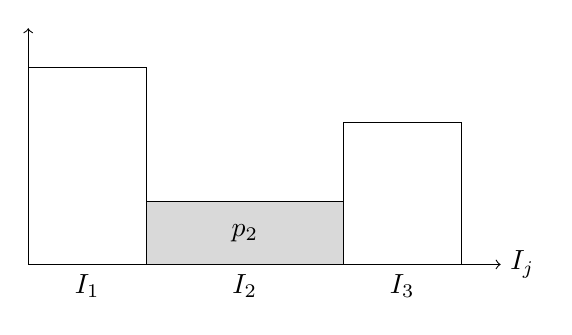
\begin{tikzpicture}\draw[->](0,0)--(6,0) node[right]{$I_j$};\draw[->](0,0)--(0,3);\draw(0,0) rectangle(1.5,2.5);\draw[fill=gray!30](1.5,0) rectangle(4,.8);\draw(4,0) rectangle(5.5,1.8);\node[below]at(.75,0){$I_1$};\node[below]at(2.75,0){$I_2$};\node[below]at(4.75,0){$I_3$};\node at(2.75,.4){$p_2$};\end{tikzpicture}\end{center}
\textbf{Valori di sintesi}: sono valori che caratterizzano i dati.
\textbf{Moda}: il valore più frequente nel dataset.
\[v_j\text{ è modale se }f_j\ge f_i\ \forall i=1,\ldots,k\quad\text{(equiv. }p_j\ge p_i\text{)}.\]
Se $f_j>f_i$ per tutti gli altri $i$ (o $p_j>p_i$), allora $v_j$ è l'unico valore modale, cioè è la moda. È utilizzata per variabili qualitative/quantitative discrete.
% Pagina originale 5
\pagina{5}Nei dati quantitativi continui al posto dei valori modali c'è/ci sono la classe moda o le classi modali, che sono quelle con densità di frequenza maggiore.
\[I_j\text{ è modale se }d_{j,A}\ge d_{i,A}\ \forall i=1,\ldots,k\quad\text{(oppure }d_{j,R}\ge d_{i,R}\text{)},\]
\[d_{j,A}=\frac{f_j}{b_j-a_j},\quad d_{j,R}=\frac{p_j}{b_j-a_j},\quad I_j=[a_j,b_j).\]
\textbf{Media}:
\[\boxed{\bar x_n=\frac1n\sum_{i=1}^n x_i},\qquad\bar x_n=\frac1n\sum_{i=1}^k v_i f_i=\sum_{i=1}^k v_i p_i.\]
Equivalente a trovare il baricentro di un'asta con $m_i=1/n$ e posizione $x_i$. Nella media tutti i valori hanno un peso. La media è sensibile ai dati anomali.

\textbf{Media pesata (ponderata)}:
\[\bar x=\sum_{i=1}^n\lambda_i x_i,\qquad\lambda_i\in(0,1],\quad\sum_{i=1}^n\lambda_i=1.\]
Per i dati raggruppati in classe la media è approssimabile come
\[\bar x_n\simeq\sum_{i=1}^k p_i\frac{a_i+b_i}{2}\quad\text{(valore medio di }I_i\text{)}.\]
La media regge le trasformazioni affini. Sia $\bar x$ media di un campione di dati $x_i$: $\bar y=a\bar x+b$ sarà la media di un campione di dati soggetti ad una trasformazione affine $y_i=ax_i+b$.
% Pagina originale 6
\pagina{6}\textbf{Dimostrazione}:
\[\bar y=\frac1n\sum_{i=1}^n(ax_i+b)=\frac1n\left[\sum_{i=1}^n ax_i+nb\right]=a\left(\frac1n\sum_{i=1}^n x_i\right)+b=a\bar x+b.\]
Esempio: $\bar T_C=\frac59(\bar T_F-32)$.

\textbf{Varianza}: indica la dispersione dei dati attorno alla media.
\[\boxed{S_n^2=\frac1{n-1}\sum_{i=1}^n(x_i-\bar x)^2}\quad\text{conoscendo un campione},\]
\[\boxed{\sigma^2=\frac1n\sum_{i=1}^n(x_i-\bar x)^2}\quad\text{conoscendo tutta la popolazione}.\]
\[S_n=\sqrt{\frac1{n-1}\sum_{i=1}^n(x_i-\bar x)^2},\qquad\sigma=\sqrt{\frac1n\sum_{i=1}^n(x_i-\bar x)^2}\quad\text{deviazione standard}.\]
La deviazione standard regge le trasformazioni lineari e non è sensibile alle traslazioni.

(1) $y_i'=ax_i\Rightarrow\bar y'=a\bar x$:
\[S_{y'}^2=\frac1{n-1}\sum_i(y_i'-\bar y')^2=\frac1{n-1}\sum_i(ax_i-a\bar x)^2=a^2\frac1{n-1}\sum_i(x_i-\bar x)^2=a^2S_x^2.\]
\[S_{y'}=|a|S_x\quad\Rightarrow\quad S_{y'}=aS_x\ (a\ge0).\]
(2) $y_i''=x_i+b\Rightarrow\bar y''=\bar x+b$:
\[S_{y''}^2=\frac1{n-1}\sum_i(y_i''-\bar y'')^2=\frac1{n-1}\sum_i(x_i+b-\bar x-b)^2=S_x^2\Rightarrow S_{y''}=S_x.\]
% Pagina originale 7
\pagina{7}\textbf{Osservazione}:
\begin{align*}S_x^2&=\frac1{n-1}\sum_i(x_i-\bar x)^2=\frac1{n-1}\sum_i(x_i^2-2x_i\bar x+\bar x^2)\\&=\frac1{n-1}\left(\sum_i x_i^2-2\bar x\sum_i x_i+n\bar x^2\right)\\&=\frac1{n-1}\left(\sum_i x_i^2-2\bar x\,n\bar x+n\bar x^2\right)=\boxed{\frac1{n-1}\left(\sum_i x_i^2-n\bar x^2\right)}.\end{align*}
\textbf{Quartili}: si basa sulla posizione dei dati in ordine crescente. Siano $x_1,\ldots,x_n$ dati non ordinati. Riordiniamo i dati $x_1\le x_2\le\cdots\le x_n$. I quartili possono essere esclusivi o inclusivi.
\[\boxed{Q_i=x_{k_i}(1-r_i)+x_{k_i+1}r_i},\qquad i\frac{n+1}{4}=k_i+r_i\quad\text{(esclusivi)},\]
con $k_i$ intero e $r_i\in\{0,\frac14,\frac24,\frac34\}$. $Q_2$ è la \textbf{mediana}:
\[M=x_{k_2}(1-r_2)+x_{k_2+1}r_2.\]
La mediana non è sensibile ai dati anomali.
\[\boxed{Q_i=x_{k_i+1}(1-r_i)+x_{k_i+2}r_i},\qquad i\frac{n-1}{4}=k_i+r_i\quad\text{(inclusivi)}.\]
I quartili sono usati per identificare dati anomali o sospetti.
\[\boxed{IQR=Q_3-Q_1\ge0}\quad\text{inter-quartile range}.\]
Dato \textbf{anomalo}: $x_i\le Q_1-3IQR$ oppure $x_i\ge Q_3+3IQR$.

Dato \textbf{sospetto}: $x_i\le Q_1-\frac32 IQR$ oppure $x_i\ge Q_3+\frac32 IQR$.
% Pagina originale 8
\pagina{8}\textbf{Box-plot (diagramma scatola e baffi)}.
\begin{center}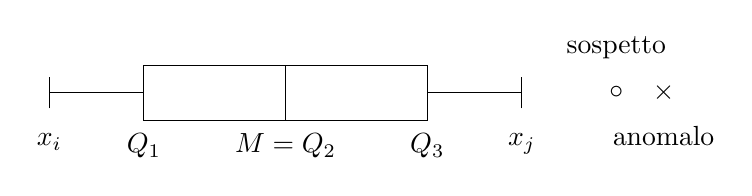
\begin{tikzpicture}[xscale=1.2]\draw(1,0)--(2,0);\draw(2,-.35)rectangle(5,.35);\draw(3.5,-.35)--(3.5,.35);\draw(5,0)--(6,0);\draw(1,-.2)--(1,.2);\draw(6,-.2)--(6,.2);\foreach\x/\s in {1/x_i,2/Q_1,3.5/M=Q_2,5/Q_3,6/x_j}{\node[below]at(\x,-.4){$\s$};}\node at(7,0){$\circ$};\node at(7.5,0){$\times$};\node[above]at(7,.3){sospetto};\node[below]at(7.5,-.3){anomalo};\end{tikzpicture}\end{center}
$x_i=\min_{x\in X}x$ non anomalo/non sospetto; $x_j=\max_{x\in X}x$ non anomalo/non sospetto: estremi dei baffi.

\textbf{Percentili}: stesso concetto dei quartili, dove l'intervallo è diviso in 100 sottointervalli e non in 4.
\[\boxed{P_i=x_{k_i}(1-r_i)+x_{k_i+1}r_i},\qquad k_i+r_i=i\frac{n+1}{100}.\]
\[P_{25}=Q_1,\quad P_{50}=Q_2=M,\quad P_{75}=Q_3,\qquad IQR=P_{75}-P_{25}.\]
\textbf{Quantili}: $k+r=(n+1)\tau$, $q_\tau=x_k(1-r)+x_{k+1}r$.

\textbf{Scatter-plot (diagramma di dispersione)}: si usa su campioni con dati bivariati, $P_i=(x_i,y_i)$.
\begin{center}\begin{tikzpicture}\draw[->](0,0)--(5,0);\draw[->](0,0)--(0,3.5);\draw[dashed](.3,.2)--(4.5,3)node[right]{retta di regressione lineare};\foreach\x/\y in {.8/.8,1.3/.7,1.7/1.5,2.2/1.8,3/2,3.8/2.8}{\fill(\x,\y)circle(2pt);}\end{tikzpicture}\end{center}
\textbf{Retta di regressione lineare}: è la retta che minimizza l'errore $|\varepsilon|^2$.
% Pagina originale 9
\pagina{9}\begin{align*}e(\alpha,\beta)&=\sum_{i=1}^n[y_i-(\alpha x_i+\beta)]^2\\&=\sum_{i=1}^n[y_i^2-2y_i(\alpha x_i+\beta)+(\alpha x_i+\beta)^2].\end{align*}
Minimizziamo $\alpha$ e $\beta$: $\nabla e=\vec0$.
\[\begin{cases}\partial e/\partial\alpha=0\\\partial e/\partial\beta=0\end{cases}\Rightarrow\begin{cases}\sum_i(-2x_i y_i+2x_i(\alpha x_i+\beta))=0\\\sum_i(-2y_i+2(\alpha x_i+\beta))=0\end{cases}\]
\[\Rightarrow\begin{cases}-\sum_i x_i y_i+\alpha\sum_i x_i^2+\beta\sum_i x_i=0\\-\sum_i y_i+\alpha\sum_i x_i+\beta n=0\end{cases}\]
Posti $Q_{xy}=\sum_i x_i y_i$, $Q_{xx}=\sum_i x_i^2$:
\[\begin{cases}-Q_{xy}+\alpha Q_{xx}+\beta n\bar x=0\\-n\bar y+\alpha n\bar x+\beta n=0\end{cases}\Rightarrow\begin{cases}Q_{xx}\alpha=Q_{xy}-\beta n\bar x\\\bar y=\alpha\bar x+\beta\end{cases}\]
\[\boxed{\alpha=\frac{Q_{xy}-n\bar x\bar y}{Q_{xx}-n\bar x^2},\qquad\beta=\bar y-\alpha\bar x}.\]
\[\beta=\bar y-\frac{Q_{xy}-n\bar x\bar y}{Q_{xx}-n\bar x^2}\bar x=\frac{Q_{xx}\bar y-n\bar x^2\bar y-Q_{xy}\bar x+n\bar x^2\bar y}{Q_{xx}-n\bar x^2}=\frac{Q_{xx}\bar y-Q_{xy}\bar x}{Q_{xx}-n\bar x^2}.\]
\[\boxed{\alpha=\frac{\operatorname{cov}(x,y)}{\operatorname{var}(x)}}=\frac{\operatorname{cov}_{x,y}}{S_x^2}=\frac{\sum_i x_i y_i-n\bar x\bar y}{\sum_i x_i^2-n\bar x^2}.\]
\textbf{Covarianza}: esprime la relazione lineare tra due variabili statistiche. La varianza è la covarianza tra le stesse variabili:
\[\operatorname{cov}_{x,x}=S_x^2,\quad\operatorname{cov}_{y,y}=S_y^2,\qquad\boxed{\operatorname{cov}_{x,y}=\frac1{n-1}\sum_{i=1}^n(x_i-\bar x)(y_i-\bar y)}.\]
% Pagina originale 10
\pagina{10}\textbf{Coefficiente di correlazione lineare}
\[\boxed{\rho=\frac{\operatorname{cov}_{x,y}}{S_xS_y}}=\frac{\sum_i x_i y_i-n\bar x\bar y}{\sqrt{(\sum_i x_i^2-n\bar x^2)(\sum_i y_i^2-n\bar y^2)}}.\]
Descrive quanto variano i dati $x_i,y_i$ in coppia rispetto a quanto variano singolarmente $x_i$ e $y_i$.
\[\alpha=\frac{\operatorname{cov}_{x,y}}{S_x^2}=\frac{\operatorname{cov}_{x,y}}{S_x^2}\frac{S_x}{S_y}\frac{S_y}{S_x}=\boxed{\rho\frac{S_y}{S_x}}.\]
Osservazione: $\rho\in[-1,1]$. $|\rho|$ indica la correlazione: $|\rho|=0$ nessuna correlazione, $|\rho|=1$ correlazione perfetta. $\operatorname{sign}(\rho)$ indica se la correlazione è crescente ($\rho>0$) o decrescente ($\rho<0$).
\[\vec w=(x_1-\bar x,\ldots,x_n-\bar x)^T,\qquad\vec v=(y_1-\bar y,\ldots,y_n-\bar y)^T.\]
\[\vec w\cdot\vec v=\sum_{i=1}^n(x_i-\bar x)(y_i-\bar y)=\operatorname{cov}_{x,y}(n-1).\]
\[\vec w\cdot\vec v=|\vec w||\vec v|\cos\theta=\sqrt{n-1}S_x\sqrt{n-1}S_y\cos\theta.\]
\[(n-1)S_xS_y\cos\theta=\operatorname{cov}_{x,y}(n-1)\Rightarrow\cos\theta=\rho_{x,y}\in[-1,1].\]
Se $\rho=0$, $\cos\theta=0$, $\theta=\pi/2+k\pi$, $\vec w\perp\vec v$.

Se $\rho=1$, $\cos\theta=1$, $\theta=0$, $\vec w=\lambda\vec v$ con $\lambda>0$:
\[y_i-\bar y=\lambda(x_i-\bar x)\Rightarrow y_i=\underbrace{\lambda}_{\alpha}x_i+\underbrace{(\bar y-\lambda\bar x)}_{\beta}.\]
% Pagina originale 11
\pagina{11}Se $\rho=-1$, $y_i=\underbrace{\lambda}_{\alpha}x_i+\underbrace{(\bar y-\lambda\bar x)}_{\beta}$, $\lambda<0$.
$\operatorname{sign}(\rho)=\operatorname{sign}(\alpha)$: il segno di $\rho$ indica la pendenza della retta ($\rho>0$ crescente, $\rho<0$ decrescente).

\textbf{Coefficiente di determinazione}
\[R^2=1-\frac{\sum_{i=1}^n[y_i-(\alpha x_i+\beta)]^2}{\sum_{i=1}^n(y_i-\bar y)^2}=\boxed{1-\frac{e(\alpha,\beta)}{S_y^2}},\qquad\boxed{R^2=\rho^2}.\]
\emph{Nota di trascrizione: qui il manoscritto denota con $S_y^2$ la somma degli scarti al quadrato, senza il fattore $1/(n-1)$.}
Se $R^2=0$, $\sum_i[y_i-(\alpha x_i+\beta)]^2/S_y^2=1$, quindi $e(\alpha,\beta)=S_y^2$.
Se $\rho=0$, $\alpha=0$, $\beta=\bar y$:
\[R^2=1-\frac{\sum_i(y_i-\beta)^2}{S_y^2}=1-\frac{\sum_i(y_i-\bar y)^2}{S_y^2}=0.\]
Se $\rho=1$, $e=0$, $R^2=1-0=1$.
\section*{Probabilità}
\textbf{Spazio degli eventi elementari (o campionario)}: $\Omega\ne\varnothing$, $\omega\in\Omega$ è un evento elementare e rappresenta una possibile osservazione dell'evento. Esempi: $\Omega=\{T,C\}$ lancio della moneta; $\Omega=\{1,2,3,4,5,6\}$ lancio di un dado.
% Pagina originale 12
\pagina{12}\textbf{Evento}: è un sottoinsieme $A\subseteq\Omega$.
\textbf{Collezione di tutti gli eventi} $\mathcal F$:
\[\mathcal F=\{A:A\subseteq\Omega\}.\]
Esempio $\Omega=\{T,C\}$, $\mathcal F_\Omega=\{\varnothing,\{T\},\{C\},\Omega\}$, $\Omega=\{T\}\cup\{C\}$; $\varnothing=\{T\}\cap\{C\}$ (esce sia T che C nello stesso lancio).

\textbf{Proprietà delle collezioni}:
\begin{enumerate}\item $\Omega\in\mathcal F$.
\item Se $A\in\mathcal F$, allora $\Omega\setminus A\in\mathcal F$.
\item $A_1,A_2,\ldots,A_n,\ldots$ successione di elementi di $\mathcal F$: $\bigcup_{i\in\mathbb N}A_i\in\mathcal F$.
\end{enumerate}
$\mathcal F$ ha una struttura algebrica $\sigma$ ($\sigma$-algebra).
Osservazioni: $\varnothing=\Omega\setminus\Omega\Rightarrow\varnothing\in\mathcal F$ (4).
\[\Omega\setminus\bigcap_{i\in\mathbb N}A_i=\bigcup_{i\in\mathbb N}(\Omega\setminus A_i)\in\mathcal F\Rightarrow\bigcap_{i\in\mathbb N}A_i\in\mathcal F\quad(5).\]
\textbf{Misura di probabilità} $\mathbb P:\mathcal F\to[0,1]$:
\begin{enumerate}\item $\mathbb P(\Omega)=1$.
\item $\mathbb P(A_i\cup A_j)=\mathbb P(A_i)+\mathbb P(A_j)$, $A_i\cap A_j=\varnothing$.
\item $\mathbb P(A_i\cup A_j)=\mathbb P(A_i)+\mathbb P(A_j)-\mathbb P(A_i\cap A_j)$ (principio di inclusione/esclusione).
\end{enumerate}
Da (2) e (3) viene fuori $\mathbb P(\varnothing)=0$.
% Pagina originale 13
\pagina{13}\textbf{Osservazione}: $\mathbb P(A\setminus B)=\mathbb P(A)-\mathbb P(B)$, $B\subset A$.
\textbf{Dimostrazione}: $A=(A\setminus B)\cup B$, $(A\setminus B)\cap B=\varnothing$.
\[\mathbb P((A\setminus B)\cup B)=\mathbb P(A\setminus B)+\mathbb P(B)=\mathbb P(A)\Rightarrow\mathbb P(A\setminus B)=\mathbb P(A)-\mathbb P(B).\]
\textbf{Osservazione}: $\mathbb P(A\cup B)=\mathbb P(A)+\mathbb P(B)-\mathbb P(A\cap B)$.
\[A\cup B=A\cup(B\setminus A),\qquad A\cap(B\setminus A)=\varnothing.\]
\[\mathbb P(A\cup B)=\mathbb P(A)+\mathbb P(B\setminus A)=\mathbb P(A)+\mathbb P(B)-\mathbb P(A\cap B).\]
Dimostrazione del principio di inclusione/esclusione.
\section*{Calcolo combinatorio}
\textbf{Disposizioni con ripetizioni}: esempio PIN di 4 cifre: $\#A=10^4=\boxed{n^k}$.

\textbf{Disposizioni senza ripetizioni}: esempio mettere 3 palline in 3 scatole, scegliendo tra 4 palline R,V,B,G ($n=4,k=3$):
\[\#A=\frac{4!}{1!}=\boxed{\frac{n!}{(n-k)!}}.\]
\textbf{Permutazioni} ($n=k$): esempio mettere 3 palline R,V,G in 3 scatole: $\#A=3!=\boxed{n!}$.
% Pagina originale 14
\pagina{14}\textbf{Combinazione semplice}: esempio mettere 3 palline su 5 in una scatola (l'ordine non importa):
\[\#A=\boxed{\binom nk}=\frac{n!}{k!(n-k)!}=\frac{5!}{3!\,2!}=10.\]
Da dove viene questa formula? Prendo ogni disposizione senza ripetizioni e mi accorgo che ci sono casi uguali (nell'esempio: stesse palline ma in ordine diverso) per il nostro calcolo. Per ogni caso ho $k!$ permutazioni. Divido $\#A_{\text{con ordine}}$ per $k!$:
\[\#A_{\text{senza ordine}}=\frac{\#A_{\text{con ordine}}}{k!}=\frac{n!}{(n-k)!}\frac1{k!}=\binom nk.\]
\textbf{Paradosso del compleanno}. $A=$ ``almeno 2 persone condividono il compleanno'', $\Omega\setminus A=$ ``tutti hanno un compleanno diverso''.
\[\mathbb P(A)=1-\mathbb P(\Omega\setminus A)=1-\frac{\#(\Omega\setminus A)}{\#\Omega}=1-\frac{365!/(365-k)!}{365^k}.\]
$\mathbb P(A)\simeq0.5037>50\%$ per $k=23$.

P.S.: $\mathbb P(X)=\#X/\#\Omega\Longleftrightarrow\mathbb P(X_1)=\mathbb P(X_2)=\cdots=\mathbb P(X_n)$. È la famosa formula ``casi favorevoli su casi totali''.

\textbf{Proprietà coefficienti binomiali}:
\[\binom nk=\binom n{n-k},\qquad\binom{n-1}{k-1}+\binom{n-1}k=\binom nk\quad\text{(triangolo di Tartaglia/Pascal)},\]
\[\sum_{i=0}^n\binom ni=2^n,\qquad(a+b)^n=\sum_{i=0}^n a^i b^{n-i}\binom ni\quad\text{(espansione polinomiale di Newton)}.\]
% Pagina originale 15
\pagina{15}\section*{Probabilità condizionata}
\[\boxed{\mathbb P(A\mid B)=\frac{\mathbb P(A\cap B)}{\mathbb P(B)}},\quad A,B\in\mathcal F,\quad\mathbb P(B)>0,\]
\[\mathbb P(A\cap B)=\mathbb P(A\mid B)\mathbb P(B).\]
Nel manoscritto: ``Se $A\subseteq B\Rightarrow\mathbb P(A\mid B)=\mathbb P(A\cap B)/\mathbb P(B)=1$''. \emph{Nota: la conclusione 1 richiede $B\subseteq A$.}
$\mathbb P(\cdot\mid B):\mathcal F\to[0,1]$ è una misura di probabilità: $\mathbb P(\Omega)=1$, $\mathbb P(\varnothing)=0$; $\mathbb P(A_1\cup A_2)=\mathbb P(A_1)+\mathbb P(A_2)-\mathbb P(A_1\cap A_2)$.
\emph{Nota: l'ultimo simbolo nell'originale è $\cup$, evidente refuso nella formula di inclusione/esclusione.}

\textbf{Teorema della probabilità totale}
\[\boxed{\mathbb P(A)=\sum_{i\in N}\mathbb P(A\mid B_i)\mathbb P(B_i)},\quad A\in\mathcal F,\]
$(B_i)_{i\in N}$ una partizione di $\Omega$: $\bigcup B_i=\Omega$, $B_i\cap B_j=\varnothing$ per $i\ne j$, $N\subseteq\mathbb N$, $\#N\ge2$.
\textbf{Dimostrazione}:
\[A=A\cap\Omega=A\cap\bigcup_{i\in N}B_i=\bigcup_{i\in N}(A\cap B_i).\]
\[\mathbb P(A)=\mathbb P\left(\bigcup_{i\in N}(A\cap B_i)\right)=\sum_{i\in N}\mathbb P(A\cap B_i)=\sum_{i\in N}\mathbb P(A\mid B_i)\mathbb P(B_i).\]
$(A\cap B_i)\cap(A\cap B_j)=\varnothing$.

\textbf{Teorema di Bayes}. Siano $A,B\in\mathcal F$, $\mathbb P(A)>0$:
\[\boxed{\mathbb P(B\mid A)=\frac{\mathbb P(A\mid B)\mathbb P(B)}{\mathbb P(A)}}.\]
Dimostrazione: $\mathbb P(B\mid A)=\mathbb P(B\cap A)/\mathbb P(A)$ e $\mathbb P(A\mid B)=\mathbb P(B\cap A)/\mathbb P(B)$; sostituendo si ottiene la formula.
% Pagina originale 16
\pagina{16}Fondamentale per l'intera probabilità e statistica. Usato nei test di screening per stabilire la probabilità della presenza di una malattia dato l'esito di un test (note la sua sensibilità e la sua specificità).

\textbf{Sensibilità}: probabilità di essere positivo se sei malato: $\mathbb P(+\mid m)=SE$.
\textbf{Specificità}: probabilità di essere negativo se sei sano: $\mathbb P(-\mid s)=SP$.
\[\mathbb P(m\mid+)=\frac{\mathbb P(+\mid m)\mathbb P(m)}{\mathbb P(+)},\qquad\mathbb P(+)=\mathbb P(+\mid m)\mathbb P(m)+\mathbb P(+\mid s)\mathbb P(s).\]
Sapendo quanto vale $\mathbb P(m)=1-\mathbb P(s)=m$:
\[\mathbb P(m\mid+)=\frac{m\mathbb P(+\mid m)}{\mathbb P(+\mid m)m+(1-m)(1-\mathbb P(-\mid s))}=\frac{mSE}{mSE+(1-m)(1-SP)}.\]
\textbf{Problema di Monty Hall}. Hai davanti a te 3 porte. Ne scegli una e ti viene aperta dal conduttore una porta. Una delle 2 porte rimaste contiene una macchina. Cambi o no la porta?

Soluzione: all'inizio ho $1/3$ di probabilità di scegliere la porta giusta, quindi $2/3$ di probabilità di aver scelto quella sbagliata. Se ho scelto quella sbagliata ($2/3$), il conduttore dovrà eliminare per forza la porta non contenente la macchina tra le 2 porte rimaste: tra le porte A e B lascerà quella con dentro la macchina. Se cambi porta hai vinto.
% Pagina originale 17
\pagina{17}Quindi, se scegli la porta sbagliata all'inizio, cambiando vinci ($p=2/3\simeq0.67$). Se invece scegli la porta giusta, cambiando porta perderai: questo accade nel $1/3$ delle volte.
Possiamo risolvere anche con il teorema di Bayes.
$A_n=$ ``la macchina è dietro la porta $n$'', $\mathbb P(A_1)=\mathbb P(A_2)=\mathbb P(A_3)=1/3$.
$B_n=$ ``il conduttore apre la porta $n$''. Ipotizzo che scelgo la porta 1:
\[\mathbb P(B_2\mid A_1)=\frac12,\qquad\mathbb P(B_2\mid A_2)=0,\qquad\mathbb P(B_2\mid A_3)=1.\]
\[\mathbb P(A_1\mid B_2)=\frac{\mathbb P(B_2\mid A_1)\mathbb P(A_1)}{\mathbb P(B_2)}=\frac{\frac12\cdot\frac13}{\mathbb P(B_2)}=\frac13.\]
\[\mathbb P(B_2)=\sum_{i=1}^3\mathbb P(B_2\mid A_i)\mathbb P(A_i)=\frac13\sum_{i=1}^3\mathbb P(B_2\mid A_i)=\frac12.\]
\[\mathbb P(A_2\mid B_2)=0,\quad\mathbb P(A_1\mid B_2)=\frac13\Rightarrow\mathbb P(A_3\mid B_2)=\frac23.\]
Nota: ricordare che $\sum_i\mathbb P(A_i\mid X)=1$ con $A_i\cap A_j=\varnothing$ per $i\ne j$.
\textbf{Eventi indipendenti}. Siano $A,B$ eventi: $\mathbb P(A\mid B)=\mathbb P(A)$ e $\mathbb P(B\mid A)=\mathbb P(B)$ indicano che $A$ e $B$ sono indipendenti.
% Pagina originale 18
\pagina{18}\[\mathbb P(A\mid B)=\mathbb P(A\cap B)\frac1{\mathbb P(B)}=\mathbb P(A)\Rightarrow\boxed{\mathbb P(A\cap B)=\mathbb P(A)\mathbb P(B)}.\]
Due eventi sono indipendenti se $\mathbb P(A\cap B)=\mathbb P(A)\mathbb P(B)$.
Due eventi sono \textbf{disgiunti} se $A\cap B=\varnothing$.
Nel manoscritto: ``2 eventi disgiunti non potranno mai essere indipendenti; disgiunti $\Rightarrow$ dipendenti''. \emph{Nota: salvo il caso di probabilità nulla.}

\textbf{Definizione}. Eventi $A_1,\ldots,A_n\in\mathcal F$ sono indipendenti se
\[\forall S\subseteq\{1,\ldots,n\}:\quad\mathbb P\left(\bigcap_{i\in S}A_i\right)=\prod_{i\in S}\mathbb P(A_i).\]
\textbf{Variabili aleatorie}. $X:\Omega\to\mathbb R$ è una funzione che verifica la proprietà: sia $(\Omega,\mathcal F,\mathbb P)$ uno spazio di probabilità; gli insiemi del tipo $\{\omega\in\Omega:X(\omega)\in I\}$ sono eventi di $\mathcal F$, quindi ha sempre senso $\mathbb P(\{\omega\in\Omega:X(\omega)\in I\})$ ($I$ intervallo aperto/chiuso, limitato/illimitato).

\textbf{Variabili aleatorie equivalenti}. Siano $X,Y$ variabili aleatorie. $X$ e $Y$ sono equivalenti se $\forall k\in\mathbb R$, $\mathbb P(\{X=k\})=\mathbb P(\{Y=k\})$.

\textbf{Legge di una variabile aleatoria}. Sia $X:\Omega\to\mathbb R$ una variabile aleatoria:
\[P_X(I)=\mathbb P(\{X\in I\})\quad\forall I\subseteq\mathbb R.\]
$P_X$ si dice ``legge'' (o ``distribuzione'') di $X$ ($X$ è distribuita con legge $P_X$).
% Pagina originale 19
\pagina{19}\textbf{Definizione}. Il range di una variabile aleatoria $X$ è l'immagine di $X$: $R(X)\equiv\operatorname{Im}(X)$.
\textbf{Definizione}. $X$ e $Y$ sono identicamente distribuite se hanno la stessa legge:
\[\mathbb P(\{X\in I\})=\mathbb P(\{Y\in I\})\quad\forall I\subseteq\mathbb R.\]
\textbf{Definizione}. $X$ e $Y$ sono indipendenti se
\[\mathbb P(\{X_1\in I_1\}\cap\{X_2\in I_2\})=\mathbb P(\{X_1\in I_1\})\mathbb P(\{X_2\in I_2\}).\]
$n$ variabili aleatorie sono indipendenti se
\[\mathbb P\left(\bigcap_{j\in J}A_j\right)=\prod_{j\in J}\mathbb P(A_j)\quad\forall J\subseteq\{1,\ldots,n\}.\]
\textbf{Definizione}. $X$ e $Y$ sono i.i.d. se sono indipendenti e identicamente distribuite.
\textbf{Definizione}. Una variabile aleatoria $X$ si dice discreta se il suo range è numerabile: $R(X)=\{x_1,x_2,\ldots,x_n\}$.
Se $X$ è discreta, per conoscere la sua legge è sufficiente conoscere $\mathbb P(\{X=x_i\})$ per $i=1,\ldots,n,\ldots$.
\section*{Valore atteso}
Sia $X$ una variabile aleatoria discreta. Il valore atteso $E(X)$ di $X$ è
\[\boxed{E(X)=\sum_{x\in R(X)}x\mathbb P(\{X=x\})}.\]
% Pagina originale 20
\pagina{20}\textbf{LOTUS (Law of the Unconscious Statistician)}.
Sia $X:\Omega\to\mathbb R$ una variabile aleatoria discreta; sia $H:\mathbb R\to\mathbb R$ una trasformazione:
\[\boxed{E(H(X))=\sum_{x\in R(X)}H(x)\mathbb P(\{X=x\})}.\]
\textbf{Teorema}. Il valore atteso è lineare: $E(aX+bY)=aE(X)+bE(Y)$.
\textbf{Dimostrazione}. Posto $H(x,y)=ax+by$,
\begin{align*}
E(aX+bY)&=\sum_{(x,y)\in R(X,Y)}H(x,y)\mathbb P(\{(X,Y)=(x,y)\})\\
&=\sum_{x,y}(ax+by)\mathbb P(\{X=x\}\cap\{Y=y\})\\
&=a\sum_{x\in R(X)}\sum_{y\in R(Y)}x\mathbb P(\{X=x\}\cap\{Y=y\})\\
&\quad+b\sum_{y\in R(Y)}\sum_{x\in R(X)}y\mathbb P(\{X=x\}\cap\{Y=y\})\\
&=a\sum_{x\in R(X)}x\mathbb P(\{X=x\})+b\sum_{y\in R(Y)}y\mathbb P(\{Y=y\})\\
&=aE(X)+bE(Y).
\end{align*}
\section*{Varianza}
Sia $X:\Omega\to\mathbb R$ una variabile aleatoria discreta. La varianza di $X$ è $\operatorname{Var}(X)=\sigma^2(X)$:
\[\boxed{\sigma^2(X)=E((X-E(X))^2)},\qquad \sigma(X)=\sqrt{\sigma^2(X)}\quad\text{(deviazione standard)}.\]
\begin{align*}
E((X-E(X))^2)&=E(X^2-2XE(X)+E(X)^2)\\
&=E(X^2)-2E(X)E(X)+E(X)^2\\
&=\boxed{E(X^2)-E(X)^2}.
\end{align*}
$E(X)$ ed $E(X)^2$ sono costanti. Osservazione: $\operatorname{Var}(X)=0\Rightarrow X=E(X)$ costante.
% Pagina originale 21
\pagina{21}\textbf{Teorema}. $\operatorname{Var}(aX+b)=a^2\operatorname{Var}(X)$.
\textbf{Dimostrazione}:
\[E([aX+b-E(aX+b)]^2)=E([aX+b-aE(X)-b]^2)=a^2E((X-E(X))^2)=a^2\operatorname{Var}(X).\]
\section*{Covarianza}
Siano $X,Y:\Omega\to\mathbb R$ variabili aleatorie. La covarianza di $X$ e $Y$ è
\begin{align*}
\operatorname{Cov}(X,Y)&=\boxed{E((X-E(X))(Y-E(Y)))}\\
&=E(XY-XE(Y)-YE(X)+E(X)E(Y))\\
&=E(XY)-E(X)E(Y)-E(Y)E(X)+E(X)E(Y)\\
&=\boxed{E(XY)-E(X)E(Y)}.
\end{align*}
\textbf{Teorema}. $\boxed{\operatorname{Var}(X+Y)=\operatorname{Var}(X)+\operatorname{Var}(Y)+2\operatorname{Cov}(X,Y)}$.
\textbf{Dimostrazione}:
\begin{align*}
E([X+Y-E(X+Y)]^2)&=E([X+Y-E(X)-E(Y)]^2)\\
&=E([X-E(X)]^2+[Y-E(Y)]^2\\
&\qquad+2(X-E(X))(Y-E(Y)))\\
&=E((X-E(X))^2)+E((Y-E(Y))^2)\\
&\qquad+2E((X-E(X))(Y-E(Y)))\\
&=\operatorname{Var}(X)+\operatorname{Var}(Y)+2\operatorname{Cov}(X,Y).
\end{align*}
\textbf{Teorema}. $X,Y$ indipendenti $\Rightarrow\operatorname{Cov}(X,Y)=0$; il viceversa non vale.
\textbf{Dimostrazione}. $\operatorname{Cov}(X,Y)=E(XY)-E(X)E(Y)=0$ perché
\begin{align*}
E(XY)&=\sum_{(x,y)\in R(X,Y)}xy\mathbb P(\{(X,Y)=(x,y)\})\\
&=\sum_{(x,y)\in R(X,Y)}xy\mathbb P(\{X=x\})\mathbb P(\{Y=y\})\\
&=\sum_{x\in R(X)}x\mathbb P(\{X=x\})\sum_{y\in R(Y)}y\mathbb P(\{Y=y\})=E(X)E(Y).
\end{align*}
% Pagina originale 22
\pagina{22}\section*{Vettori aleatori}
È una mappa $X=(X_1,X_2,\ldots,X_n):\Omega\to\mathbb R^n$, dove $X_1,\ldots,X_n$ sono variabili aleatorie.
La legge congiunta è la misura di probabilità su $\mathbb R^n$ data da $P_X(E)=\mathbb P(\{X\in E\})$, $E\subseteq\mathbb R^n$.
Le leggi $P_{X_1},\ldots,P_{X_n}$ delle componenti $X_1,\ldots,X_n$ sono dette leggi marginali.
\textbf{Definizione}. Un vettore aleatorio è discreto se ogni sua componente $X_i$ è discreta.
\[R(X)=R(X_1)\times R(X_2)\quad\text{(prodotto cartesiano, come indicato nell'originale)}.\]
\begin{center}\begin{tabular}{c|ccccc}$X_2\backslash X_1$&0&1&2&3&$\cdots$\\\hline
0&$p_{00}$&$p_{10}$&$p_{20}$&$p_{30}$&\\
1&$p_{01}$&$p_{11}$&$p_{21}$&$p_{31}$&\\
2&$p_{02}$&$p_{12}$&$p_{22}$&$p_{32}$&\\
3&$p_{03}$&$p_{13}$&$p_{23}$&$p_{33}$&
\end{tabular}\end{center}
Con $p_{xy}=\mathbb P(\{(X_1,X_2)=(x,y)\})$:
\begin{align*}
\mathbb P(\{X_1=\bar x\})&=\sum_{y\in R(X_2)}\mathbb P(\{X_1=\bar x\}\mid\{X_2=y\})\mathbb P(\{X_2=y\})\\
&=\sum_{y\in R(X_2)}\mathbb P(\{(X_1,X_2)=(\bar x,y)\})=\sum_{y\in R(X_2)}p_{\bar xy}.
\end{align*}
\textbf{Definizione}. $X,Y$ sono vettori aleatori indipendenti se
\[\mathbb P(\{X\in E\}\cap\{Y\in F\})=\mathbb P(\{X\in E\})\mathbb P(\{Y\in F\}),\quad\forall E,F\subseteq\mathbb R^n.\]
$n$ vettori aleatori sono indipendenti se
\[\mathbb P\left(\bigcap_{i=1}^n\{X_i\in E_i\}\right)=\prod_{i=1}^n\mathbb P(\{X_i\in E_i\})\quad\forall E_i\subseteq\mathbb R^n.\]
Per considerare gruppi non globali basta prendere $E_i=\mathbb R^n$ per gli indici esclusi. Esempio: $X_1,X_3,X_7\Rightarrow E_2,E_4,E_5,E_6=\mathbb R^n$.
% Pagina originale 23
\pagina{23}\textbf{Proposizione}. Siano $X_1,\ldots,X_n,Y_1,\ldots,Y_m$ indipendenti. Allora $X=(X_1,\ldots,X_n)$ e $Y=(Y_1,\ldots,Y_m)$ sono indipendenti.
\textbf{Dimostrazione}. $E=I_1\times\cdots\times I_n$, $F=J_1\times\cdots\times J_m$:
\begin{align*}
\mathbb P(\{X\in E\}\cap\{Y\in F\})&=\mathbb P\left(\bigcap_{i=1}^n\{X_i\in I_i\}\cap\bigcap_{j=1}^m\{Y_j\in J_j\}\right)\\
&=\mathbb P\left(\bigcap_{i=1}^n\{X_i\in I_i\}\right)\mathbb P\left(\bigcap_{j=1}^m\{Y_j\in J_j\}\right)\\
&=\mathbb P(\{X\in E\})\mathbb P(\{Y\in F\}).
\end{align*}
\section*{Funzioni di vettori aleatori}
$X=(X_1,\ldots,X_n):\Omega\to\mathbb R^n$. Consideriamo $H:\mathbb R^n\to\mathbb R$: $H(X_1,\ldots,X_n)$ è una variabile aleatoria.
\textbf{Proposizione}. Se $X=(X_1,\ldots,X_n)$ e $Y=(Y_1,\ldots,Y_m)$ sono vettori aleatori indipendenti, e $H:\mathbb R^n\to\mathbb R$, $G:\mathbb R^m\to\mathbb R$ sono funzioni di vettori aleatori, allora $H(X_1,\ldots,X_n)$ e $G(Y_1,\ldots,Y_m)$ sono indipendenti.
\textbf{Dimostrazione}:
\begin{align*}
\mathbb P(\{H(X)\in I\}\cap\{G(Y)\in J\})&=\mathbb P(\{X\in H^{-1}(I)\}\cap\{Y\in G^{-1}(J)\})\\
&=\mathbb P(\{X\in H^{-1}(I)\})\mathbb P(\{Y\in G^{-1}(J)\})\\
&=\mathbb P(\{H(X)\in I\})\mathbb P(\{G(Y)\in J\}).
\end{align*}
\section*{Leggi note}
Ci sono varie leggi probabilistiche note. Appartengono a due classi principali: 1. discrete; 2. continue.
% Pagina originale 24
\pagina{24}\section*{Leggi discrete}
\textbf{Legge di Bernoulli}. $X\sim Be(p)$, $p\in(0,1)$. Descrive il successo/insuccesso.
\[\boxed{\mathbb P(\{X=0\})=1-p,\quad\mathbb P(\{X=1\})=p},\qquad\boxed{E(X)=p,\quad\operatorname{Var}(X)=p(1-p)}.\]
\begin{center}\begin{tikzpicture}[x=2cm,y=2cm]\draw[->](-.3,0)--(1.5,0);\draw[->](-.3,0)--(-.3,1);\draw (0,0) rectangle (.08,.33);\draw (1,0) rectangle (1.08,.67);\node[below]at(0,0){0};\node[below]at(1,0){1};\node at(.7,.95){$p=0.67$};\end{tikzpicture}\end{center}
\textbf{Dimostrazione}: $E(X)=\sum_{x\in R(X)}x\mathbb P(\{X=x\})=p$;
\[\operatorname{Var}(X)=E(X^2)-E(X)^2=\sum_{x\in R(X)}x^2\mathbb P(\{X=x\})-p^2=p-p^2.\]
\textbf{Legge binomiale}. $X\sim B(n,p)$, $n>0$, $p\in(0,1)$. Descrive il numero di successi $k$ in $n$ tentativi. È la somma di $X_i\sim Be(p)$ i.i.d., $i\in\{1,\ldots,n\}$.
\[\boxed{\mathbb P(\{X=k\})=\binom nkp^k(1-p)^{n-k}},\quad k\in[0,n],\qquad\boxed{E(X)=np,\quad\operatorname{Var}(X)=np(1-p)}.\]
\begin{center}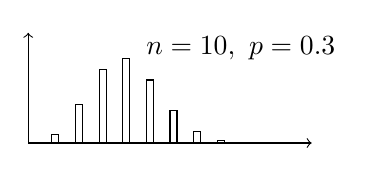
\begin{tikzpicture}[x=.3cm,y=4cm]\draw[->](-1,0)--(11,0);\draw[->](-1,0)--(-1,.35);\foreach \k/\h in {0/.028,1/.121,2/.233,3/.267,4/.200,5/.103,6/.037,7/.009,8/.001,9/.0001,10/.00001}{\draw(\k,0)rectangle(\k+.3,\h);}\node at(8,.3){$n=10,\ p=0.3$};\end{tikzpicture}\end{center}
\textbf{Dimostrazione}: $E(X)=\sum_{i=1}^nE(X_i)=np$; $\operatorname{Var}(X)=\sum_{i=1}^n\operatorname{Var}(X_i)=np(1-p)$, poiché $X_i$ indipendenti implica covarianza nulla.
Siano $X\sim B(n,p)$ e $Y\sim B(m,p)$: $X+Y\sim B(n+m,p)$.
\textbf{Dimostrazione}: $X+Y=\sum_{i=1}^nX_i+\sum_{j=1}^mY_j=\sum_{i=1}^{n+m}X_i\sim B(n+m,p)$, con addendi $Be(p)$.
\emph{Nota: l'indipendenza di $X$ e $Y$ è necessaria e sottintesa nel manoscritto.}
% Pagina originale 25
\pagina{25}\textbf{Legge di Poisson}. $X\sim\mathcal P(\lambda)$, $\lambda>0$. Descrive il numero di successi in ``tanti'' tentativi indipendenti, con una media finita.
\[\boxed{\mathbb P(\{X=k\})=\frac{\lambda^k}{k!}e^{-\lambda}},\quad\lambda=np,\qquad\boxed{E(X)=\lambda,\quad\operatorname{Var}(X)=\lambda}.\]
\begin{center}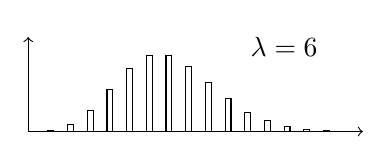
\begin{tikzpicture}[x=.25cm,y=6cm]\draw[->](-1,0)--(16,0);\draw[->](-1,0)--(-1,.2);\foreach \k/\h in {0/.0025,1/.015,2/.045,3/.089,4/.134,5/.161,6/.161,7/.138,8/.103,9/.069,10/.041,11/.023,12/.011,13/.005,14/.002}{\draw(\k,0)rectangle(\k+.3,\h);}\node at(12,.18){$\lambda=6$};\end{tikzpicture}\end{center}
\textbf{Dimostrazione}. $X_n\sim B(n,p)$; vogliamo $\lim_{n\to\infty}\mathbb P(\{X_n=k\})=\lambda^ke^{-\lambda}/k!$.
\begin{align*}
\mathbb P(\{X_n=k\})&=\binom nkp^k(1-p)^{n-k}\\
&=\frac{n!}{k!(n-k)!}\left(\frac\lambda n\right)^k\left(1-\frac\lambda n\right)^{n-k}\\
&=\frac{\lambda^k}{n^k}\frac{n(n-1)\cdots(n-k+1)}{k!}\left(1-\frac\lambda n\right)^n\left(1-\frac\lambda n\right)^{-k}\\
&=\frac{\lambda^k}{k!}\frac{n(n-1)\cdots(n-k+1)}{\underbrace{n\cdots n}_{k\text{ volte}}}\left(1-\frac\lambda n\right)^{-k}\left(1-\frac\lambda n\right)^n\\
&\longrightarrow\frac{\lambda^k}{k!}e^{-\lambda}.
\end{align*}
Infatti, con $y=-n/\lambda$, $\lim_{n\to\infty}(1-\lambda/n)^n=\lim_{y\to-\infty}(1+1/y)^{-\lambda y}=e^{-\lambda}$.
\begin{align*}
E(X)&=\sum_{k=0}^\infty k\mathbb P(\{X=k\})=\sum_{k=0}^\infty ke^{-\lambda}\frac{\lambda^k}{k!}\\
&=e^{-\lambda}\sum_{k=1}^\infty\frac{\lambda^k}{(k-1)!}=\lambda e^{-\lambda}\sum_{k=1}^\infty\frac{\lambda^{k-1}}{(k-1)!}=\lambda e^{-\lambda}e^\lambda=\lambda.
\end{align*}
Si usa $\sum_{k=0}^\infty a^k/k!=e^a$. Inoltre $np(1-p)=\lambda(1-\lambda/n)\to\lambda$.
\begin{align*}
\operatorname{Var}(X)&=E((X-E(X))^2)=E(X^2)-E(X)^2\\
&=\sum_{k=0}^\infty k^2e^{-\lambda}\frac{\lambda^k}{k!}-\lambda^2
=\lambda e^{-\lambda}\sum_{k=1}^\infty k\frac{\lambda^{k-1}}{(k-1)!}-\lambda^2\\
&=\lambda e^{-\lambda}\sum_{h=0}^\infty(h+1)\frac{\lambda^h}{h!}-\lambda^2=\lambda^2+\lambda-\lambda^2=\lambda.
\end{align*}
% Pagina originale 26
\pagina{26}\textbf{Teorema}. $X\sim\mathcal P(\lambda)$, $Y\sim\mathcal P(\mu)$ indipendenti $\Rightarrow X+Y\sim\mathcal P(\lambda+\mu)$.
\textbf{Dimostrazione}:
\begin{align*}
\mathbb P(\{X+Y=k\})&=\sum_{h=0}^k\mathbb P(\{X=h\}\cap\{Y=k-h\})\\
&=\sum_{h=0}^k\mathbb P(\{X=h\})\mathbb P(\{Y=k-h\})\\
&=\sum_{h=0}^ke^{-\lambda}\frac{\lambda^h}{h!}e^{-\mu}\frac{\mu^{k-h}}{(k-h)!}\\
&=\frac{e^{-(\lambda+\mu)}}{k!}\sum_{h=0}^k\binom kh\lambda^h\mu^{k-h}=e^{-(\lambda+\mu)}\frac{(\lambda+\mu)^k}{k!}.
\end{align*}
L'ultima somma è il polinomio di Newton.
\textbf{Legge geometrica}. $X\sim Geo(p)$, $p\in(0,1)$. Descrive il primo successo in tentativi indipendenti con probabilità $p$.
\[\boxed{\mathbb P(\{X=k\})=(1-p)^{k-1}p},\qquad\boxed{E(X)=\frac1p,\quad\operatorname{Var}(X)=\frac{1-p}{p^2}}.\]
\begin{center}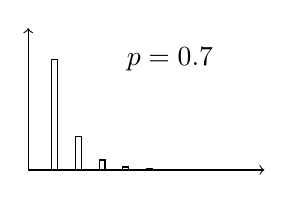
\begin{tikzpicture}[x=.3cm,y=2cm]\draw[->](0,0)--(10,0);\draw[->](0,0)--(0,.9);\foreach \k/\h in {1/.7,2/.21,3/.063,4/.019,5/.006,6/.002,7/.0005}{\draw(\k,0)rectangle(\k+.25,\h);}\node at(6,.7){$p=0.7$};\end{tikzpicture}\end{center}
\textbf{Dimostrazione}. Posto $q=1-p$,
\begin{align*}
E(X)&=\sum_{k=1}^\infty k\mathbb P(\{X=k\})=p\sum_{k=1}^\infty k(1-p)^{k-1}\\
&=p\sum_{k=1}^\infty kq^{k-1}=p\sum_{k=1}^\infty\frac{d}{dq}q^k=p\frac{d}{dq}\sum_{k=0}^\infty q^k\\
&=p\frac{d}{dq}\frac1{1-q}=\frac{p}{(1-q)^2}=\frac1p.
\end{align*}
$q^0=1$ è costante e la sua derivata è nulla.
\begin{align*}
\operatorname{Var}(X)&=E(X^2)-E(X)^2=\sum_{k=1}^\infty k^2\mathbb P(\{X=k\})-\frac1{p^2}\\
&=p\sum_{k=1}^\infty k^2q^{k-1}-\frac1{p^2}=p\frac d{dq}\sum_{k=1}^\infty kq^k-\frac1{p^2}\\
&=p\frac d{dq}\left(q\sum_{k=0}^\infty\frac d{dq}q^k\right)-\frac1{p^2}
=p\frac d{dq}\frac q{(1-q)^2}-\frac1{p^2}\\
&=p\frac{(1-q)^2+2q(1-q)}{(1-q)^4}-\frac1{(1-q)^2}\\
&=\frac{p+2(1-p)}{p^2}-\frac1{p^2}=\frac{p+2-2p-1}{p^2}=\frac{1-p}{p^2}.
\end{align*}
% Pagina originale 27
\pagina{27}La legge geometrica gode di \textbf{assenza di memoria} (è l'unica legge discreta con questa proprietà):
\[\boxed{\mathbb P(\{X>m+n\}\mid\{X>n\})=\mathbb P(\{X>m\})}.\]
\textbf{Dimostrazione}:
\begin{align*}
\mathbb P(\{X>m+n\}\mid\{X>n\})&=\frac{\mathbb P(\{X>m+n\}\cap\{X>n\})}{\mathbb P(\{X>n\})}\\
&=\frac{\mathbb P(\{X>m+n\})}{\mathbb P(\{X>n\})}=\frac{(1-p)^{m+n}}{(1-p)^n}=(1-p)^m=\mathbb P(\{X>m\}).
\end{align*}
\textbf{Proposizione}. $\mathbb P(\{X>k\})=(1-p)^k$.
\textbf{Dimostrazione}, posto $j=h-k-1$:
\[\mathbb P(\{X>k\})=\sum_{h=k+1}^\infty\mathbb P(\{X=h\})=p\sum_{h=k+1}^\infty(1-p)^{h-1}\]\[=p\sum_{j=0}^\infty(1-p)^{j+k}=p(1-p)^k\sum_{j=0}^\infty(1-p)^j=(1-p)^k.\]
\section*{Leggi continue}
Una variabile aleatoria $X:\Omega\to\mathbb R$ ha funzione di densità di probabilità (f.d.p.) $f_X:\mathbb R\to[0,+\infty)$ se
\[\mathbb P(\{X\in I\})=\int_I f_X(x)\,dx.\]
Osservazioni: $\int_{\mathbb R}f_X(x)\,dx=1$; $\int_a^a f_X(x)\,dx=0=\mathbb P(\{X=a\})$.
La funzione di distribuzione cumulativa (F.d.c.) è
\[F_X(x)=\int_{-\infty}^x f_X(t)\,dt=\mathbb P(\{X\le x\}).\]
Osservazioni: $F_X(x)\to0$ per $x\to-\infty$; $F_X(x)\to1$ per $x\to+\infty$; $x_1\le x_2\Rightarrow F_X(x_1)\le F_X(x_2)$.
\emph{Nota: nel manoscritto l'ultima implicazione è disegnata in entrambe le direzioni; il viceversa non vale in generale.}
% Pagina originale 28
\pagina{28}Se $X$ ha f.d.p. $f_X\in C^0(\mathbb R)$ (a tratti), allora $\boxed{F_X(x)=\int_{-\infty}^x f_X(t)\,dt}$ è derivabile e $F_X'(x)=f_X(x)$ per il teorema fondamentale del calcolo integrale (nei punti di continuità).
\textbf{Valore atteso}:\[\boxed{E(X)=\int_{\mathbb R}xf_X(x)\,dx}.\] Con $f_X$ f.d.p. di $X:\Omega\to\mathbb R$.
\textbf{Varianza}: $\boxed{\operatorname{Var}(X)=E(X^2)-E(X)^2}$.
\section*{Leggi continue}
\textbf{Legge uniforme}. $X\sim U(a,b)$, $a<b$:
\[\boxed{f_X(x)=\frac1{b-a}},\quad x\in(a,b),\qquad \boxed{E(X)=\frac{a+b}2,\quad\operatorname{Var}(X)=\frac{(b-a)^2}{12}}.\]
\begin{center}\begin{tikzpicture}\draw[->](-1,0)--(4,0);\draw[->](0,-.3)--(0,2);\draw(1,0)--(1,1)--(3,1)--(3,0);\draw[dashed](0,1)--(1,1);\node[left]at(0,1){$1/(b-a)$};\node[below]at(1,0){$a$};\node[below]at(3,0){$b$};\end{tikzpicture}\end{center}
\textbf{Dimostrazione}:
\[E(X)=\int_a^b\frac{x}{b-a}\,dx=\frac{b^2-a^2}{b-a}\frac12=\frac{a+b}2.\]
\begin{align*}
\operatorname{Var}(X)&=E(X^2)-E(X)^2=\int_a^b\frac{x^2}{b-a}\,dx-\frac{(a+b)^2}4\\
&=\frac13\frac{b^3-a^3}{b-a}-\frac14(a^2+2ab+b^2)\\
&=\frac13(b^2+a^2+ab)-\frac14(a^2+2ab+b^2)\\
&=\frac1{12}(4b^2+4a^2+4ab-3a^2-3b^2-6ab)\\
&=\frac1{12}(a^2-2ab+b^2)=\frac{(b-a)^2}{12}.
\end{align*}
% Pagina originale 29
\pagina{29}\textbf{Legge esponenziale}. $X\sim Exp(\lambda)$, $\lambda>0$. Descrive i tempi di attesa con proprietà particolari.
\[\boxed{f_X(x)=\lambda e^{-\lambda x}},\quad x>0,\qquad\boxed{E(X)=\frac1\lambda,\quad\operatorname{Var}(X)=\frac1{\lambda^2}}.\]
\begin{center}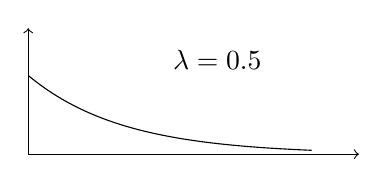
\begin{tikzpicture}[x=.6cm,y=2cm]\draw[->](0,0)--(7,0);\draw[->](0,0)--(0,.8);\draw[domain=0:6,samples=50]plot(\x,{.5*exp(-.5*\x)});\node at(4,.6){$\lambda=0.5$};\end{tikzpicture}\end{center}
\textbf{Dimostrazione}:
\begin{align*}
E(X)&=\int_0^\infty xf_X(x)\,dx=\int_0^\infty x\lambda e^{-\lambda x}\,dx\\
&=\left[-xe^{-\lambda x}\right]_0^\infty+\int_0^\infty e^{-\lambda x}\,dx=\left[-\frac1\lambda e^{-\lambda x}\right]_0^\infty=\frac1\lambda.
\end{align*}
$\operatorname{Var}(X)=E(X^2)-E(X)^2=2/\lambda^2-1/\lambda^2=1/\lambda^2$, perché
\begin{align*}
E(X^2)&=\int_0^\infty x^2f_X(x)\,dx=\left[-x^2e^{-\lambda x}\right]_0^\infty+\int_0^\infty2xe^{-\lambda x}\,dx\\
&=2\left(\left[-\frac{x}{\lambda}e^{-\lambda x}\right]_0^\infty+\int_0^\infty\frac1\lambda e^{-\lambda x}\,dx\right)=\frac2{\lambda^2}.
\end{align*}
Osservazione: $\mathbb P(\{X>t\})=\int_t^\infty\lambda e^{-\lambda x}\,dx=e^{-\lambda t}$.
Osservazione: $\mathbb P(\{X>t+z\}\mid\{X>z\})=\mathbb P(\{X>t\})$.
La legge esponenziale è l'unica legge continua che gode di assenza di memoria.
\textbf{Dimostrazione}:
\[\mathbb P(\{X>t+z\}\mid\{X>z\})=\frac{\mathbb P(\{X>t+z\}\cap\{X>z\})}{\mathbb P(\{X>z\})}\]\[=\frac{\mathbb P(\{X>t+z\})}{\mathbb P(\{X>z\})}=\frac{e^{-\lambda(t+z)}}{e^{-\lambda z}}=e^{-\lambda t}=\mathbb P(\{X>t\}).\]
\section*{Vettori aleatori continui}
Un vettore aleatorio ha f.d.p. congiunta $f_{X,Y}(x,y)$ se
% Pagina originale 30
\pagina{30}\[\mathbb P(\{(X,Y)\in E\})=\iint_E f(x,y)\,dx\,dy.\]
$f_X$ e $f_Y$ si dicono marginali:
\[f_X(x)=\int_{-\infty}^{+\infty}f_{X,Y}(x,y)\,dy,\qquad F_X(x)=\int_{-\infty}^x\int_{-\infty}^{+\infty}f_{X,Y}(t,y)\,dy\,dt.\]
\section*{Variabili aleatorie indipendenti}
$X$ e $Y$ sono indipendenti se $\boxed{f_{X,Y}(x,y)=f_X(x)f_Y(y)}$.
\textbf{Dimostrazione}:
\begin{align*}
\mathbb P(\{(X,Y)\in(-\infty,x]\times(-\infty,y]\})&=\int_{-\infty}^x\int_{-\infty}^y f_{X,Y}(t,u)\,du\,dt\\
&=\mathbb P(\{X\le x\}\cap\{Y\le y\})\\
&=\int_{-\infty}^xf_X(t)\,dt\int_{-\infty}^yf_Y(u)\,du\\
&=\mathbb P(\{X\le x\})\mathbb P(\{Y\le y\}).
\end{align*}
Derivando in $x$ e $y$ otteniamo $f_{X,Y}(x,y)=f_X(x)f_Y(y)$.
\textbf{Teorema}. Siano $X$ e $Y$ indipendenti con f.d.p. $f_X(x)$ e $f_Y(y)$:
\begin{align*}
F_{X+Y}(z)&=\mathbb P(\{X+Y\le z\})=\int_{-\infty}^z f_{X+Y}(t)\,dt\\
&=\mathbb P(\{(X,Y)\in E\}),\quad E=\{(x,y)\in\mathbb R^2:x+y\le z\}\\
&=\int_{-\infty}^{+\infty}\left(\int_{-\infty}^{z-x}f_{X,Y}(x,y)\,dy\right)dx\\
&=\int_{-\infty}^{+\infty}\left(\int_{-\infty}^{z}f_{X,Y}(x,u-x)\,du\right)dx\\
&=\int_{-\infty}^z\left(\int_{-\infty}^{+\infty}f_{X,Y}(x,u-x)\,dx\right)du\\
&=\int_{-\infty}^z f_{X+Y}(t)\,dt.
\end{align*}
\begin{center}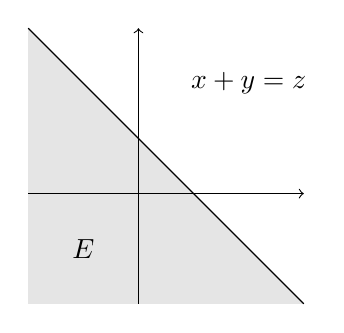
\begin{tikzpicture}[scale=.7]\fill[gray!20](-2,-2)--(3,-2)--(-2,3)--cycle;\draw[->](-2,0)--(3,0);\draw[->](0,-2)--(0,3);\draw(-2,3)--(3,-2);\node at(2,2){$x+y=z$};\node at(-1,-1){$E$};\end{tikzpicture}\end{center}
\[F'_{X+Y}(z)=\boxed{f_{X+Y}(z)}=\int_{-\infty}^{+\infty}f_{X,Y}(x,z-x)\,dx=\boxed{\int_{-\infty}^{+\infty}f_X(x)f_Y(z-x)\,dx}=[f_X*f_Y](z).\]
$f_X*f_Y$ è la \textbf{convoluzione}.

% Pagina originale 31
\pagina{31}
\subsection*{Convoluzione}
\[ (f_X*f_Y)(z)=\int_{-\infty}^{+\infty}f_X(x)f_Y(z-x)\,dx. \]
\textbf{Osservazione.} Calcoliamo con la convoluzione $X_1+X_2$, con $X_1,X_2\sim\operatorname{Exp}(\lambda)$ indipendenti:
\begin{align*}
f_{X_1+X_2}(z)&=\int_{-\infty}^{+\infty}f_{X_1}(x)f_{X_2}(z-x)\,dx\\
&=\int_0^z\lambda e^{-\lambda x}\lambda e^{-\lambda(z-x)}\,dx
=\int_0^z\lambda^2e^{-\lambda z}\,dx=z\lambda^2e^{-\lambda z},\\
f_{X_1+X_2+X_3}(z)&=(f_{X_1+X_2}*f_{X_3})(z)=\cdots=\lambda^3\frac{z^2}{2}e^{-\lambda z}.
\end{align*}
\subsection*{Legge Gamma}
$X\sim\operatorname{Gamma}(\alpha,\lambda)$, $\alpha>0$, $\lambda>0$. È la somma di $\alpha$ esponenziali $X_i\sim\operatorname{Exp}(\lambda)$:
\[ \sum_{i=1}^{\alpha}X_i=X\sim\operatorname{Gamma}(\alpha,\lambda). \]
\[\boxed{f_X(x)=\frac{\lambda^\alpha}{\Gamma(\alpha)}x^{\alpha-1}e^{-\lambda x}},\qquad
\Gamma(\alpha)=\int_0^{+\infty}y^{\alpha-1}e^{-y}\,dy=(\alpha-1)!\quad(\alpha\in\mathbb N).\]
\[\boxed{\mathbb E(X)=\frac\alpha\lambda,\qquad\operatorname{Var}(X)=\frac\alpha{\lambda^2}.}\]
\begin{center}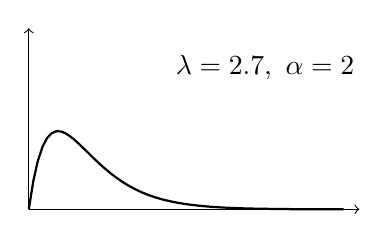
\begin{tikzpicture}[x=1cm,y=1cm]
\draw[->](0,0)--(4.2,0);\draw[->](0,0)--(0,2.3);
\draw[thick,domain=0:4,samples=70] plot (\x,{7.29*\x*exp(-2.7*\x)});
\node at (3,1.8) {$\lambda=2.7,\ \alpha=2$};
\end{tikzpicture}\end{center}
\textbf{Dimostrazione 1.}
\[\mathbb E(X)=\mathbb E\left(\sum_{i=1}^{\alpha}X_i\right)=\sum_{i=1}^{\alpha}\mathbb E(X_i)=\frac\alpha\lambda,\qquad
\operatorname{Var}(X)=\operatorname{Var}\left(\sum_{i=1}^{\alpha}X_i\right)=\sum_{i=1}^{\alpha}\operatorname{Var}(X_i)=\frac\alpha{\lambda^2}.\]
\textbf{Dimostrazione 2.}
\begin{align*}
\mathbb E(X)&=\int_{-\infty}^{+\infty}x\frac{\lambda^\alpha}{\Gamma(\alpha)}x^{\alpha-1}e^{-\lambda x}\,dx\\
&=\int_0^{+\infty}\frac{\lambda^\alpha}{\Gamma(\alpha)}x^{(\alpha-1)+1}e^{-\lambda x}\,dx\\
&=\frac{\lambda^\alpha}{\Gamma(\alpha)}\frac{\Gamma(\alpha+1)}{\lambda^{\alpha+1}}
\underbrace{\int_0^{+\infty}\frac{\lambda^{\alpha+1}}{\Gamma(\alpha+1)}x^{(\alpha+1)-1}e^{-\lambda x}\,dx}_{1}=\frac\alpha\lambda,\\
\operatorname{Var}(X)&=\mathbb E(X^2)-\mathbb E(X)^2
=\frac{\alpha^2+\alpha}{\lambda^2}-\frac{\alpha^2}{\lambda^2}=\frac\alpha{\lambda^2}.
\end{align*}
% Pagina originale 32
\pagina{32}
\begin{align*}
\mathbb E(X^2)&=\int_0^{+\infty}x^2\frac{\lambda^\alpha}{\Gamma(\alpha)}x^{\alpha-1}e^{-\lambda x}\,dx\\
&=\frac{\lambda^\alpha}{\Gamma(\alpha)}\frac{\Gamma(\alpha+2)}{\lambda^{\alpha+2}}
\int_0^{+\infty}\frac{\lambda^{\alpha+2}}{\Gamma(\alpha+2)}x^{(\alpha+2)-1}e^{-\lambda x}\,dx
=\frac{\alpha(\alpha+1)}{\lambda^2}.
\end{align*}
\textbf{Teorema.} $X\sim\operatorname{Gamma}(\alpha,\lambda)$, $Y\sim\operatorname{Gamma}(\beta,\lambda)$:
\[X+Y\sim\operatorname{Gamma}(\alpha+\beta,\lambda).\]
\subsection*{Legge normale}
$X\sim\mathcal N(\mu,\sigma^2)$, $\mu\in\mathbb R$, $\sigma^2\ge0$.
La somma di $n>30$ variabili $X_i$ i.i.d. porta ad una legge normale (teorema del limite centrale).
\[\boxed{f_X(x)=\frac1{\sigma\sqrt{2\pi}}e^{-\frac12((x-\mu)/\sigma)^2}}\quad X\sim\mathcal N(\mu,\sigma^2),\]
\[f_X(x)=\frac1{\sqrt{2\pi}}e^{-x^2/2}\quad X\sim\mathcal N(0,1).\]
\[\boxed{\mathbb E(X)=\mu,\quad\operatorname{Var}(X)=\sigma^2}\quad\text{per definizione}.\]
\begin{center}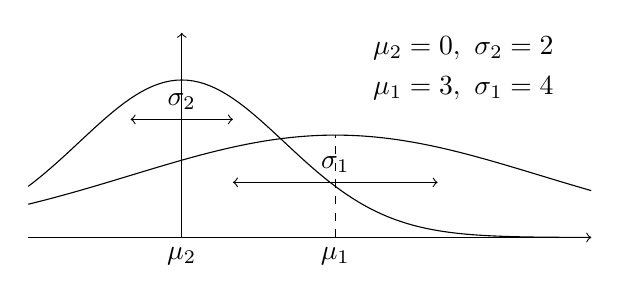
\begin{tikzpicture}[x=.65cm,y=1cm]
\draw[->](-3,0)--(8,0);\draw[->](0,0)--(0,2.6);
\draw[domain=-3:8,samples=100] plot(\x,{2*exp(-\x*\x/8)});
\draw[domain=-3:8,samples=100] plot(\x,{1.3*exp(-(\x-3)*(\x-3)/32)});
\draw[dashed](3,0)--(3,1.3);\node[below] at(0,0){$\mu_2$};\node[below] at(3,0){$\mu_1$};
\node at(5.5,2.4){$\mu_2=0,\ \sigma_2=2$};\node at(5.5,1.9){$\mu_1=3,\ \sigma_1=4$};
\draw[<->](-1,1.5)--(1,1.5) node[midway,above]{$\sigma_2$};\draw[<->](1,.7)--(5,.7)node[midway,above]{$\sigma_1$};
\end{tikzpicture}\end{center}
\[F_X(x)=\Phi(x)\quad\text{per }X\sim\mathcal N(0,1).\]
\textit{z-value}: $z=(x-\mu)/\sigma$ (quante deviazioni standard dista $x$ da $\mu$).
\textbf{Proprietà.} $X\sim\mathcal N(\mu,\sigma^2)$, $Y\sim\mathcal N(\nu,\tau^2)$:
\begin{gather*}
X+Y\sim\mathcal N(\mu+\nu,\sigma^2+\tau^2),\quad X+k\sim\mathcal N(\mu+k,\sigma^2),\\
aX\sim\mathcal N(a\mu,a^2\sigma^2),\quad aX+k\sim\mathcal N(a\mu+k,a^2\sigma^2).
\end{gather*}
% Pagina originale 33
\pagina{33}
\section*{Statistica inferenziale}
\textbf{Definizione.} Un vettore aleatorio $X'=(X_1,X_2,\ldots,X_n)$ composto da variabili aleatorie i.i.d. si chiama \emph{campione casuale}.

\textbf{Definizione.} I dati di un campione casuale $(X_1,X_2,\ldots,X_n)$ sono\[ (x_1,x_2,\ldots,x_n)\in R(X_1,X_2,\ldots,X_n).\]
$X$ è definita da parametri $\theta\in\Theta$.
\[X\sim\operatorname{Be}(p)\Rightarrow\theta=p,\quad\Theta=[0,1];\qquad
X\sim B(n,p)\Rightarrow\theta=(n,p),\quad\Theta=\mathbb N\times[0,1].\]
\subsection*{Obiettivo della statistica inferenziale}
Preso un campione casuale $(X_1,X_2,\ldots,X_n)$ della popolazione $X$, definita dai parametri $\theta\in\Theta$, l'obiettivo della statistica inferenziale è quello di ottenere informazioni sulla popolazione a partire dai dati $(x_1,\ldots,x_n)$ (questo processo è detto ``di inferenza'').

\textbf{Definizione.} Sia $(X_1,\ldots,X_n)$ un campione casuale. Una \emph{statistica} costruita a partire dal campione è una variabile aleatoria $H(X_1,\ldots,X_n)$.

\textbf{Esempio.} La media campionaria è la statistica $\overline X_n$:
\[\boxed{\overline X_n=\frac1n\sum_{i=1}^n X_i}.\]
$\overline x_n$ è la realizzazione di $\overline X_n$ calcolata sui dati:
\[\overline x_n=\frac1n\sum_{i=1}^n x_i.\]
Se la popolazione $X$ è definita da parametri $\theta\in\Theta$, $h(\theta)$ il parametro da stimare e $H(X_1,\ldots,X_n)$ ha lo scopo di stimare $h(\theta)$, allora $H(X_1,\ldots,X_n)$ è uno \emph{stimatore} di $h(\theta)$.
% Pagina originale 34
\pagina{34}
\textbf{Definizione.} Uno stimatore si dice \emph{corretto} se $H(X_1,\ldots,X_n)$ ha come valore atteso $h(\theta)$:
\[\mathbb E\bigl(H(X_1,\ldots,X_n)\bigr)=h(\theta).\]
$H(x_1,\ldots,x_n)$ si dice \emph{stima puntuale} di $h(\theta)$.

\textbf{Esempio.} La varianza campionaria è la statistica $S_n^2$:
\[\boxed{S_n^2=\frac1{n-1}\sum_i(X_i-\overline X_n)^2}.\]
\[s_n^2=\frac1{n-1}\sum_i(x_i-\overline x_n)^2\quad\text{è la realizzazione sui dati}.\]
\textbf{Osservazione.}
\[\boxed{\mathbb E(\overline X_n)=\mu,\qquad\operatorname{Var}(\overline X_n)=\frac{\sigma^2}{n}\ne\sigma^2}.\]
Con $n\to+\infty$, $\operatorname{Var}(\overline X_n)\to0$ (sempre più certa): legge dei grandi numeri.
\subsection*{Legge dei grandi numeri}
Siano $X_1,\ldots,X_n$ i.i.d. con $\mathbb E(X_i)=\mu$ e $\operatorname{Var}(X_i)=\sigma^2$:
\[\forall\varepsilon>0,\qquad\lim_{n\to+\infty}\mathbb P\{|\overline X_n-\mu|<\varepsilon\}=1.\]
\textbf{Dimostrazione.}
\[\mathbb P\{|\overline X_n-\mu|>\varepsilon\}=1-\mathbb P\{|\overline X_n-\mu|<\varepsilon\}\longrightarrow0.\]
Ponendo $Y=(\overline X_n-\mu)^2$:
\begin{align*}
\mathbb P\{|\overline X_n-\mu|>\varepsilon\}&=\mathbb P\{(\overline X_n-\mu)^2>\varepsilon^2\}
=\int_{\varepsilon^2}^{+\infty}f_Y(y)\,dy\\
&=\int_{\varepsilon^2}^{+\infty}\frac{\varepsilon^2}{\varepsilon^2}f_Y(y)\,dy
\le\frac1{\varepsilon^2}\int_{\varepsilon^2}^{+\infty}y f_Y(y)\,dy\\
&\le\frac1{\varepsilon^2}\int_0^{+\infty}y f_Y(y)\,dy
=\frac1{\varepsilon^2}\mathbb E(Y)=\frac1{\varepsilon^2}\mathbb E\bigl((\overline X_n-\mu)^2\bigr)\\
&=\frac1{\varepsilon^2}\left[\operatorname{Var}(\overline X_n-\mu)+\mathbb E(\overline X_n-\mu)^2\right]
=\frac1{\varepsilon^2}\left(\frac{\sigma^2}{n}+0^2\right)=\frac{\sigma^2}{\varepsilon^2 n}\longrightarrow0.
\end{align*}
% Pagina originale 35
\pagina{35}
Dalla legge dei grandi numeri nasce la \emph{simulazione di Montecarlo}.
Sapendo che con $n\to+\infty$ tentativi $\overline X_n\to\mu$, possiamo usare un calcolatore per simulare $n$ tentativi e trovare $\mu$.
\textbf{Esempio.} Simulazione Montecarlo per $\pi$.
\begin{center}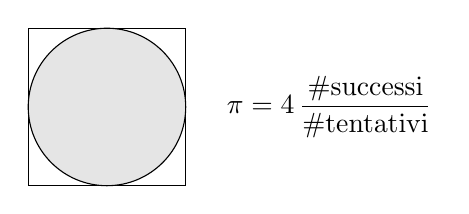
\begin{tikzpicture}\draw (0,0) rectangle(2,2);\draw[fill=gray!20](1,1)circle(1);\node[right]at(2.4,1){$\pi=4\,\dfrac{\#\text{successi}}{\#\text{tentativi}}$};\end{tikzpicture}\end{center}
\[\#\text{successi}=A_{\circ}=\pi(1/2)^2=\pi/4,\quad\#\text{tentativi}=A_{\square}=1^2=1,\quad\mu\to\pi/4.\]
\subsection*{Teorema del limite centrale}
Sia $X$ popolazione con $\mathbb E(X)=\mu$ e $\operatorname{Var}(X)=\sigma^2$, $X_1,\ldots,X_n$ i.i.d.:
\[\lim_{n\to+\infty}\mathbb P\left\{\frac{\overline X_n-\mu}{\sigma/\sqrt n}\le z\right\}=\Phi(z)=\frac1{\sqrt{2\pi}}\int_{-\infty}^z e^{-t^2/2}\,dt.\]
Applicabile per $n\ge30$ senza aver bisogno di conoscere la legge di $X_i$.
\subsection*{Intervalli di confidenza (I.C.)}
Un I.C. con livello di confidenza $\beta$ è un intervallo aleatorio $[U_n,V_n]$, dove $U_n=u_n(X_1,\ldots,X_n)$ e $V_n=v_n(X_1,\ldots,X_n)$ sono statistiche, tali che
\[\boxed{\beta=\mathbb P\{U_n\le h(\theta)\le V_n\}}.\]
\textbf{Esempio.} $h(\theta)=\mu$ ($\sigma$ noto):
\begin{align*}
\beta&=\mathbb P\{U_n\le\mu\le V_n\}=\mathbb P\{-V_n\le-\mu\le-U_n\}\\
&=\mathbb P\left\{\frac{\overline X_n-V_n}{\sigma/\sqrt n}\le
\underbrace{\frac{\overline X_n-\mu}{\sigma/\sqrt n}}_{Z\sim\mathcal N(0,1)}\le\frac{\overline X_n-U_n}{\sigma/\sqrt n}\right\}.
\end{align*}
% Pagina originale 36
\pagina{36}
\begin{align*}
\beta&=1-\mathbb P\left(\left\{Z\le\frac{\overline X_n-V_n}{\sigma/\sqrt n}\right\}\cup
\left\{Z\ge\frac{\overline X_n-U_n}{\sigma/\sqrt n}\right\}\right)\\
&=1-2\underbrace{\mathbb P\{Z\ge z_{\alpha/2}\}}_{\alpha/2},\qquad\alpha=1-\beta.
\end{align*}
\[(1-2\alpha/2=1-\alpha=\beta).\]
\begin{gather*}
\frac{\overline X_n-V_n}{\sigma/\sqrt n}=-z_{\alpha/2}\Rightarrow V_n=\overline X_n+\frac\sigma{\sqrt n}z_{\alpha/2},\\
\frac{\overline X_n-U_n}{\sigma/\sqrt n}=z_{\alpha/2}\Rightarrow U_n=\overline X_n-\frac\sigma{\sqrt n}z_{\alpha/2},\\
\boxed{\mathrm{I.C.}=\left[\overline X_n-z_{\alpha/2}\frac\sigma{\sqrt n},\ \overline X_n+z_{\alpha/2}\frac\sigma{\sqrt n}\right]},\\
z_{\alpha/2}=\Phi^{-1}(1-\alpha/2),\qquad[z_x=\Phi^{-1}(1-x)],\qquad[\Phi(x)+\Phi(-x)=1].
\end{gather*}
\begin{center}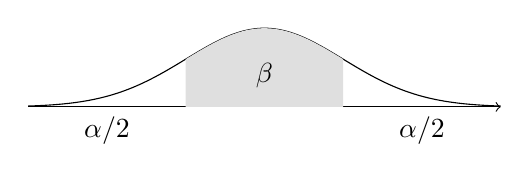
\begin{tikzpicture}[x=1cm,y=1cm]\draw[->](-3,0)--(3,0);\draw[domain=-3:3,samples=80]plot(\x,{exp(-\x*\x/2)});\fill[gray!25,domain=-1:1,samples=40](-1,0)--plot(\x,{exp(-\x*\x/2)})--(1,0)--cycle;\node at(0,.4){$\beta$};\node[below]at(-2,0){$\alpha/2$};\node[below]at(2,0){$\alpha/2$};\end{tikzpicture}\end{center}
\textbf{Esempio.} $h(\theta)=\sigma^2$:
\begin{align*}
\beta&=\mathbb P\{U_n\le\sigma^2\le V_n\}=\mathbb P\{1/V_n\le1/\sigma^2\le1/U_n\}\\
&=\mathbb P\left\{\frac{(n-1)S_n^2}{V_n}\le\underbrace{\frac{(n-1)S_n^2}{\sigma^2}}_{Z\sim\chi^2(n-1)}\le\frac{(n-1)S_n^2}{U_n}\right\}.
\end{align*}
\begin{gather*}
\frac{(n-1)S_n^2}{V_n}=\chi^2_{n-1,1-\alpha/2}\Rightarrow V_n=\frac{(n-1)S_n^2}{\chi^2_{n-1,1-\alpha/2}},\\
\frac{(n-1)S_n^2}{U_n}=\chi^2_{n-1,\alpha/2}\Rightarrow U_n=\frac{(n-1)S_n^2}{\chi^2_{n-1,\alpha/2}},\\
\boxed{\mathrm{I.C.}=\left[\frac{(n-1)S_n^2}{\chi^2_{n-1,\alpha/2}},\ \frac{(n-1)S_n^2}{\chi^2_{n-1,1-\alpha/2}}\right]}.
\end{gather*}
\emph{Nota di trascrizione: nell'originale, due indici nella derivazione di $V_n$ sembrano scritti $1+\alpha/2$; il riquadro finale riporta $1-\alpha/2$. Qui è seguito il riquadro. I quantili sono indicati secondo la convenzione di coda destra.}
\begin{center}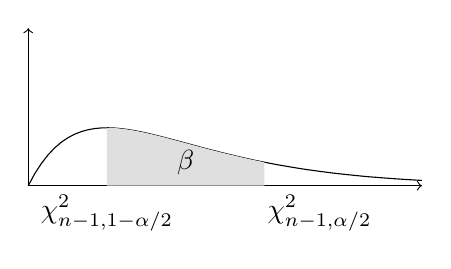
\begin{tikzpicture}\draw[->](0,0)--(5,0);\draw[->](0,0)--(0,2);\draw[domain=0:5,samples=60]plot(\x,{2*\x*exp(-\x)});\fill[gray!25,domain=1:3,samples=30](1,0)--plot(\x,{2*\x*exp(-\x)})--(3,0)--cycle;\node at(2,.3){$\beta$};\node[below]at(1,0){$\chi^2_{n-1,1-\alpha/2}$};\node[below]at(3.7,0){$\chi^2_{n-1,\alpha/2}$};\end{tikzpicture}\end{center}
% Pagina originale 37
\pagina{37}
\textbf{Esempio.} $h(\theta)=\mu$ ($\sigma$ non noto):
\[\beta=\mathbb P\{U_n\le\mu\le V_n\}
=\mathbb P\left\{\frac{\overline X_n-V_n}{S_n/\sqrt n}\le\underbrace{\frac{\overline X_n-\mu}{S_n/\sqrt n}}_{\sim t(n-1)}\le\frac{\overline X_n-U_n}{S_n/\sqrt n}\right\}.\]
\section*{Leggi continue per analisi inferenziale}
\subsection*{Chi-quadro}
$X\sim\chi^2(n)$:
\[\chi^2(n)=\operatorname{Gamma}(n/2,1/2),\qquad
\boxed{f_X(x)=\frac{\lambda^{n/2}}{\Gamma(n/2)}x^{n/2-1}e^{-x/2}}\quad(\lambda=1/2).\]
\begin{center}\begin{tikzpicture}\draw[->](0,0)--(5,0);\draw[->](0,0)--(0,2);\draw[domain=0.01:5,samples=80]plot(\x,{1.5*sqrt(\x)*exp(-\x/2)});\node at(4,1.5){$n=3$};\end{tikzpicture}\end{center}
\textbf{Osservazione.} $\sum_{i=1}^n X_i^2=Z\sim\operatorname{Gamma}(n/2,1/2)$, $X_i\sim\mathcal N(0,1)$.
\textbf{Dimostrazione.} $f_{Z^2}(x)=?$ (qui $Z$ indica una normale standard).
\begin{align*}
\mathbb P\{Z^2\le x\}&=0\quad\forall x\le0,\\
\mathbb P\{Z^2\le x\}&=\mathbb P\{-\sqrt x\le Z\le\sqrt x\}=2\mathbb P\{0\le Z\le\sqrt x\}\\
&=2\int_0^{\sqrt x}\frac1{\sqrt{2\pi}}e^{-t^2/2}\,dt
\quad(y=t^2)\\
&=2\int_0^x\frac1{\sqrt{2\pi}}\frac1{2\sqrt y}e^{-y/2}\,dy=F_{Z^2}(x),\\
F'_{Z^2}(x)&=f_{Z^2}(x)=\frac1{\sqrt{2\pi}}\frac1{\sqrt x}e^{-x/2}
=\frac{(1/2)^{1/2}}{\underbrace{\Gamma(1/2)}_{\sqrt\pi}}x^{1/2-1}e^{-x/2}.
\end{align*}
\textbf{Perché si usa?}
\begin{align*}
S_n^2&=\frac1{n-1}\sum_{i=1}^n(X_i-\overline X_n)^2\\
&=\frac1{n-1}\sum_{i=1}^n\left[(X_i-\mu)^2+(\overline X_n-\mu)^2-2(X_i-\mu)(\overline X_n-\mu)\right]\\
&=\frac1{n-1}\left[\sum_{i=1}^n(X_i-\mu)^2+n(\overline X_n-\mu)^2-2(\overline X_n-\mu)(n\overline X_n-n\mu)\right].
\end{align*}
% Pagina originale 38
\pagina{38}
\begin{align*}
S_n^2&=\frac1{n-1}\left[\sum_{i=1}^n(X_i-\mu)^2-n(\overline X_n-\mu)^2\right],\\
(n-1)S_n^2&=\sum_{i=1}^n(X_i-\mu)^2-n(\overline X_n-\mu)^2,\\
\frac{(n-1)S_n^2}{\sigma^2}+n\left(\frac{\overline X_n-\mu}{\sigma}\right)^2&=\sum_{i=1}^n\left(\frac{X_i-\mu}{\sigma}\right)^2,\\
\frac{(n-1)S_n^2}{\sigma^2}+\underbrace{\left(\frac{\overline X_n-\mu}{\sigma/\sqrt n}\right)^2}_{Z_0^2,\ Z_0\sim\mathcal N(0,1)}&=\sum_{i=1}^n\underbrace{\left(\frac{X_i-\mu}{\sigma}\right)^2}_{Z_i^2,\ Z_i\sim\mathcal N(0,1)},\\
\frac{(n-1)S_n^2}{\sigma^2}+Z_0^2&=\sum_{i=1}^n Z_i^2.
\end{align*}
\begin{gather*}
Z_0^2\sim\chi^2(1)=\operatorname{Gamma}(1/2,1/2),\quad Z_i^2\sim\chi^2(1)=\operatorname{Gamma}(1/2,1/2),\\
\sum Z_i^2\sim\chi^2(n)=\operatorname{Gamma}(n/2,1/2),\\
\Rightarrow\frac{(n-1)S_n^2}{\sigma^2}\sim\operatorname{Gamma}((n-1)/2,1/2)=\chi^2(n-1).
\end{gather*}
\subsection*{t-Student}
$X\sim t(n)$:
\[X=\frac Z{\sqrt{Q_n/n}},\qquad Z\sim\mathcal N(0,1),\quad Q_n\sim\chi^2(n).\]
\[\boxed{f_X(x)=\frac{\Gamma((n+1)/2)}{\sqrt{n\pi}\,\Gamma(n/2)}\frac1{(1+x^2/n)^{(n+1)/2}}}.\]
\[n\to+\infty\Rightarrow X\sim t(n)\approx\mathcal N(0,1).\]
\textbf{Perché si usa?}
\begin{align*}
\frac{\overline X_n-\mu}{S_n/\sqrt n}&=\frac{\overline X_n-\mu}{\sigma/\sqrt n}\frac\sigma{S_n}
=\underbrace{Z}_{\sim\mathcal N(0,1)}\frac1{\sqrt{S_n^2/\sigma^2}}\frac{\sqrt{n-1}}{\sqrt{n-1}}\\
&=Z\frac{\sqrt{n-1}}{\sqrt{(n-1)S_n^2/\sigma^2}}
=\frac Z{\sqrt{Q_{n-1}/(n-1)}}\sim t(n-1),\quad Q_{n-1}=\frac{(n-1)S_n^2}{\sigma^2}\sim\chi^2(n-1).
\end{align*}
% Pagina originale 39
\pagina{39}
\subsection*{Intervallo di confidenza unilaterale}
\[\boxed{\beta=\mathbb P\{U_n\le h(\theta)\}}\quad\text{limite inferiore di confidenza }U_n,\]
\[\boxed{\beta=\mathbb P\{h(\theta)\le V_n\}}\quad\text{limite superiore di confidenza }V_n.\]
\textbf{Nota.} In questo caso viene preso $z_\alpha$ e non $z_{\alpha/2}$.
\subsection*{Test di ipotesi}
Si parte da un'ipotesi nulla $H_0:h(\theta)\in E_0$ e si verifica che l'ipotesi alternativa $H_1:h(\theta)\in E_1$, con $E_0\cap E_1=\varnothing$, è rifiutabile o accettabile secondo il livello di significatività $\alpha\in(0,1)$.
\textbf{Errori.}
\begin{center}\begin{tabular}{c|cc}&$H_0$ vera&$\overline H_0$ vera\\\hline
Accettare $H_0$&corretto&II tipo\\Rifiutare $H_0$&I tipo&corretto\end{tabular}\end{center}
I tipo: $\mu=3$ ($H_0$), ma pensiamo che $\mu>3$ ($H_1$).
II tipo: $\mu>3$ ($H_1$), ma pensiamo che $\mu=3$ ($H_0$).
Il livello di significatività $\alpha$ è la probabilità di commettere un errore del I tipo.
\[\boxed{R_c=\{(x_1,\ldots,x_n)\in R(X_1,\ldots,X_n):\overline x_n>\mu_0+\delta\}},\]
\[\boxed{\alpha=\mathbb P\{(X_1,\ldots,X_n)\in R_c\}}\quad\text{essendo vera }\mu=\mu_0.\]
\begin{align*}
\alpha&=\mathbb P\{\overline X_n>\mu_0+\delta\}
=\mathbb P\left\{\frac{\overline X_n-\mu}{\sigma/\sqrt n}>\frac{\mu_0-\mu}{\sigma/\sqrt n}+\frac\delta{\sigma/\sqrt n}\right\}\\
&=\mathbb P\left\{\underbrace{Z}_{\sim\mathcal N(0,1)}>\frac\delta{\sigma/\sqrt n}\right\}\quad(\mu=\mu_0).
\end{align*}
\[\frac\delta{\sigma/\sqrt n}=z_\alpha\Rightarrow\delta=\frac\sigma{\sqrt n}z_\alpha.\]
Se $\overline x_n>\mu_0+\delta=\mu_0+\frac\sigma{\sqrt n}z_\alpha$, allora $H_0$ è rifiutata.
% Pagina originale 40
\pagina{40}
\textbf{Osservazione.} Se $H_0$ è rifiutata con livello di significatività $\alpha'$, allora $H_0$ è rifiutata con $\alpha>\alpha'$.
\subsection*{p-value}
Il p-value è il più piccolo livello di significatività $\alpha$ per cui i dati permettono di rifiutare l'ipotesi nulla $H_0$.
\[\forall\alpha>\text{p-value}:H_0\text{ è rifiutata};\qquad\forall\alpha<\text{p-value}:H_0\text{ è accettata}.\]
\begin{align*}
\text{p-value}&=\inf\left\{\alpha\in(0,1):\overline x_n>\mu_0+\frac\sigma{\sqrt n}z_\alpha\right\}\\
&=\inf\left\{\alpha\in(0,1):\underbrace{\frac{\overline x_n-\mu_0}{\sigma/\sqrt n}}_{\text{z-score}}>z_\alpha\right\}\\
&=\inf_{\alpha\in(0,1)}\left\{\Phi(z_\alpha)<\Phi\left(\frac{\overline x_n-\mu_0}{\sigma/\sqrt n}\right)\right\}\\
&=\inf_{\alpha\in(0,1)}\left\{1-\alpha<\Phi\left(\frac{\overline x_n-\mu_0}{\sigma/\sqrt n}\right)\right\}\\
&=\inf_{\alpha\in(0,1)}\left\{\alpha>1-\Phi\left(\frac{\overline x_n-\mu_0}{\sigma/\sqrt n}\right)\right\}
=1-\Phi\left(\frac{\overline x_n-\mu_0}{\sigma/\sqrt n}\right)=\Phi(-\text{z-value}).
\end{align*}

\end{document}
